\documentclass[]{article}
\usepackage{graphicx}
\usepackage{float}
\usepackage{amsmath,amssymb,amsthm} % For including math equations, theorems, symbols, etc
\usepackage{subfig}
\graphicspath{{Figures/}} 
\usepackage{hyperref}
\PassOptionsToPackage{dvipsnames}{xcolor}
\RequirePackage{xcolor} % [dvipsnames]
\definecolor{CTsemi}{gray}{0.55} % chapter numbers will be semi transparent .5 .55 .6 .0
\definecolor{CTcitation}{rgb}{0,0.5,0} % WebGreen
\definecolor{CTurl}{named}{Maroon} % Maroon
\definecolor{CTtitle}{named}{Maroon} % Maroon {cmyk}{0, 0.87, 0.68, 0.32}
\definecolor{CTlink}{named}{RoyalBlue} % RoyalBlue {cmyk}{1, 0.50, 0, 0}
\definecolor{halfgray}{gray}{0.55} % chapter numbers will be semi transparent .5 .55 .6 .0
\definecolor{webgreen}{rgb}{0,0.5,0}
\definecolor{webbrown}{rgb}{0.6,0,0}
\hypersetup{
	colorlinks=true,
	linkcolor=RoyalBlue,
	filecolor=magenta,      
	urlcolor=cyan,
	pdfkeywords={}
	breaklinks=true, bookmarks=true,bookmarksnumbered,
	urlcolor=webbrown, citecolor=webgreen, % Link colors
	pdftitle={}, % PDF title
	pdfauthor={\textcopyright}, % PDF Author
	pdfsubject={}, % PDF Subject
	pdfkeywords={}, % PDF Keywords
	pdfcreator={pdfLaTeX}, % PDF Creator
	pdfproducer={LaTeX with hyperref and ClassicThesis} % PDF producer
}

%opening
\title{Bayesian Evidence Synthesis:opioid crisis}
\author{Hyeongcheol Park* \& Paul Gustafson* \& Micheal A Irvine*\textsuperscript{1}}

\begin{document}
%\renewcommand{\sectionmark}[1]{\markright{\spacedlowsmallcaps{#1}}}
\maketitle{}
\tableofcontents % Print the table of contents
\listoffigures % Print the list of figures
\listoftables % Print the list of tables


\begin{abstract}

\end{abstract}

\section{Introduction}
The opioid crisis is a major issue in North America  including Canada. There were 1,490 deaths and 15,598 paramedic- attended overdose events during 2017 alone. \cite{Irvine:modelling} (need to know about bib in latex, change statistics to 2018 later) The goal of this project is to apply Bayesian evidence synthesis to understand better the opoid crisis in Vancouver, Canada.  \\

[Need to give a backstory-why isn't this observable? The number of overdoses] [specify a geographic area]
\\

All examples here were performed in Python 3.7 using the library pyMC (reference) and JAGS (reference). Training was performed using No U-Turn Sampling (NUTS) over two chains with 1000 iterations (is it sample size?). Fitting was performed on a GHz Intel Core i5 with 8GM of LPDD3 RAM and typically had wall times under ten minutes. Data processing was carried out using the Pandas and SciPy library [reference]. Data visualization was performed using the libraries Seaborn and Matplotlib [ref]. Code for all examples in this study are provided. \\

[explain Bayesian statistics, MCMC and related topics]

\section{methods}

\normalsize
The number of overdoses is our ultimate interest of estimation.  Let $O_t$ the number of overdoses in a given month $t$. Suppose there was a survey  conducted to estimate the proportion of ambulance call $p_A$ among the overdoses. $p_A$ is assumed constant across time for simplicity. Let $n_{A}$ the sample size of the survey and $x_{A}$ to be the total number who confirmed they did call ambulance. It is assumed that $x_{A}$ follows a Binomial distribution:

\begin{equation}
\label{ambulance}
\left.\begin{aligned}
x_{A} \sim Bin(n_{A},p_{A})\end{aligned}\right.
\text{		ambulance call-outs model}
\end{equation}

The total overdoses need to be modeled. The simplest conceptual model is to take an underlying log-rate $z_t$ that is independent and identically distributed across months according to a normal distribution with mean $\mu$ and variance $\sigma^2$. \cite{Irvine:modelling} Denote $\lambda_{t}^{OD}$ the rate of overdose at time $t$. It is assumed that the total overdose $O_t$ follows Poisson distribution where the population of the region of interest is $N$. 
[Give a graphical model representation? state that(?)]

\begin{equation}
\label{overdose}
\left.\begin{aligned}
z_{t} \sim N(\mu, \sigma^{2}) \\
\lambda_{t}^{OD} = \exp(z_{t})\\
O_{t} \sim Poi(\lambda_{t}^{OD}N) 
\end{aligned}\right\} 
\text{		overdose model} 
\end{equation}

Estimation of $O_t$ is not straightforward since none of the variables ($\mu$, $\sigma$, $N$) determining $O_t$  is known. Hence $O_t$ should be inferred from using $U_t$ and \(p_A\), where $p_A$ is the ambulance call out rate and \(U_t\) is the number of  ambulance-attended overdoses at a time point $t$. In general, the data of ambulance-attended overdoses \(U_t\) can be obtained. It is assumed that  \(U_t\) follows Binomial distribution: 
\begin{equation}
\label{over_amb}
\left.
U_t \sim Bin(O_t, p_A)
\right.
\end{equation}

Now $O_t$ can be estimated as $p_A$ can be infered by survey data and the data regarding $U_t$ is given. We suggest a simple model as a start where the model only combines Ambulance Call-outs Model (\ref{ambulance}) and Overdose Model (\ref{overdose}). 

The next step is to run some simulations to figure out how different types of inputs lead some changes of output. To do so, the simple model is illustrated below.\\

\subsection{Simulation}

\normalsize 
The first simulation simplifies the assumptions of variables as much as possible; We assumed $N= 10000, n_{A}=1000$. Note that the population size, N,  is unknown in reality but it is assumed known for the investigator here for simplicity. The assumptions will change later to see the impact of the likelihood over the posterior distributions of variables of interest; The total population size for a region, N, could vary over time or it can be staritified for a better realization of the real world. We vary the survey size  as $n_{A}=100$ or $n_{A}=10000$.  \\

\subsubsection{Likelihood}

\normalsize 
There exist two data sets; survey data ($n_A, x_A$), and ambulance attended overdose data ($U_t$). The two data sets are simulated as follows. 
The true value of $p_A$ was set $p_A=0.8$ for the survey data.
It is assumed that the data was collected for a year (t=1,2,3, ..., 12) and 
$x_t$ values were independentally generated from the Binomial distribution (\ref{ambulance}).  In terms of overdose data, It is assumed that the true values of parameters for overdose model were $\mu=\log0.05,\ \sigma=1$.
The vector of $O_t$ was generated following the overdose model (\ref{overdose}). The vector of $U_t$ was generated from the Binomial relation of the two variables ($\ref{over_amb}$). The two generated vectors have the same length with the survey data (t=1,2,3, ..., 12). [Delete: Then the 12 sueveys were combined into a single survey since $p_A$ is assumed fixed across time in this contexts.] Note that only $U_t$ and $x_t$ are known as the likelihood and $p_A$ needs to be estimated first so as to estimate $O_t$ which is the ultimate interest of the research.\\


\subsubsection{Prior Distributions}
\normalsize Noninformative prior distributions are presumed as a start for simplicity. 

\begin{equation}
\label{nonin_prior_amb}
p(p_A) \sim Beta(1,1)
\text{			noninformative prior of ambulance model}
\end{equation} 

\begin{equation}
\label{noninprior_over}
\left.\begin{aligned}
\mu \sim U(-10,0)\\
\sigma \sim U(0,5)
\end{aligned}\right\} 
\text{			noninformative prior of overdose model}
\end{equation}

This leads the posterior distribution of variables of interest to heavily depend on the likelihood. Later, the noninformative priors will be changed and the impact of the changes over posteriors will be investigated. \\

\subsection{Early Result } 

The result from the simple case scenario is illustrated below.

\subsubsection{Posterior Distribution}


Figure \ref{pst_ot} is the boxplot of posterior samples of $O_t$. It is shown that our posterior estimates of  $O_t$ are fairly accurate since (1) the boxplots contain actual values of $O_t$ within their interquartile range (IQR) and (2) the ranges of IQR and 95\% range seem narrow. Notice that the range of the boxplot from a higher $O_t$ values (t=1, 7, 11) is wider than the other ranges of the boxplots from smaller estimates of $O_t$ (all t values but 1, 7, 11)\\

\begin{figure}[h]
	\centering
	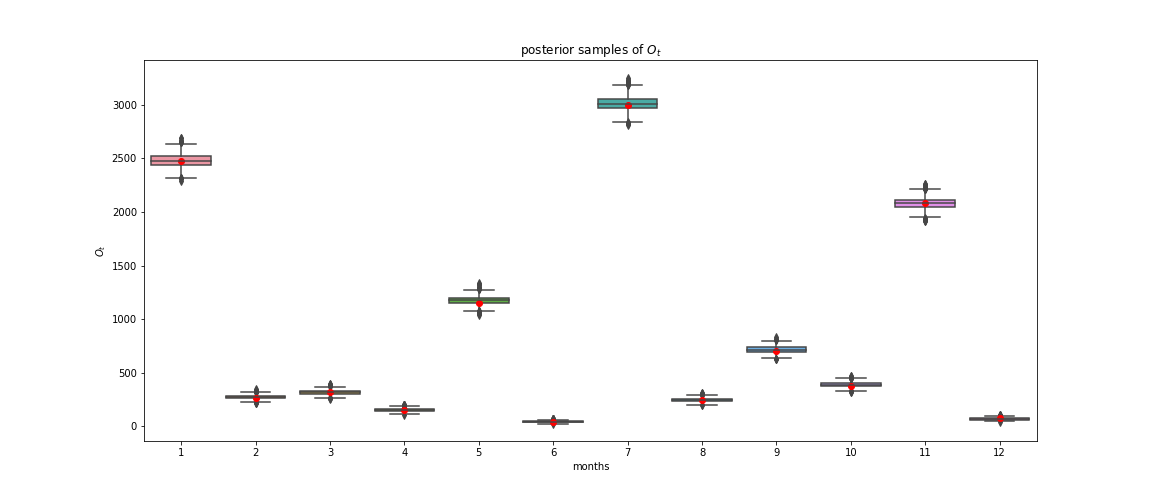
\includegraphics[width=1\linewidth]{Figures/earlyresult1_ot.png}
	\caption{Boxplot of posterior samples of $O_t$ (2000 samples for each month) with actual data points of simulated $O_t$ values. The simulated values are shown as red dots.}
	\label{pst_ot}
\end{figure}

\newpage
\subsubsection{Posterior Predictive Check}

Figure \ref{ppc_ut} is the boxplot of posterior predictive samples of $U_t$. It is shown that the posterior predictive estimates of $U_t$ is failry accurate with the same two reasons regarding the accuracy of the posterior distribution of $O_t$. It is more obvious here that the range of the boxplots from higher $O_t$ values (t=1, 7, 11) is wider than the other ranges of the boxplots from smaller estimates of $O_t$ (all t values but 1,7, 11). Notice that the relative ranges of figure \ref{ppc_ut} follow the ones of figure \ref{pst_ot}; For months where $U_t$ values are higher, the values of $O_t$ are also higher than the average (t=1, 7, 11)\\

\begin{figure}[htb]
	\centering
	\subfloat[ppc of $U_t$]{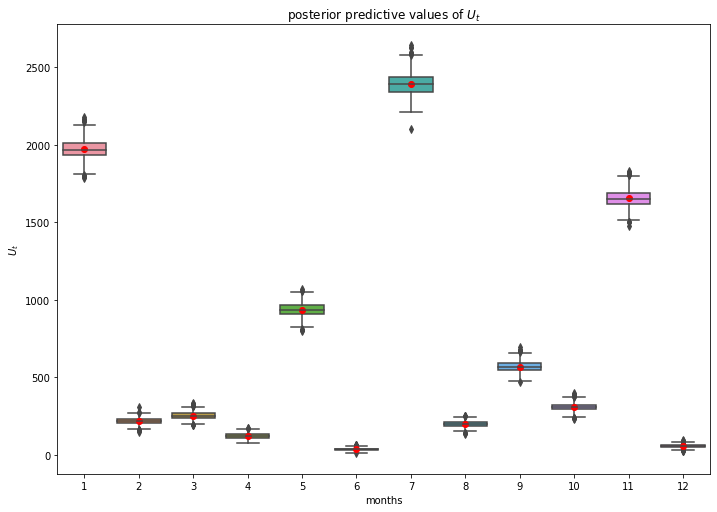
\includegraphics[width=.50\columnwidth]{Figures/early_r_ppc1_ut.png}\label{ppc_ut}}
	\subfloat[ppc of $p_A$]{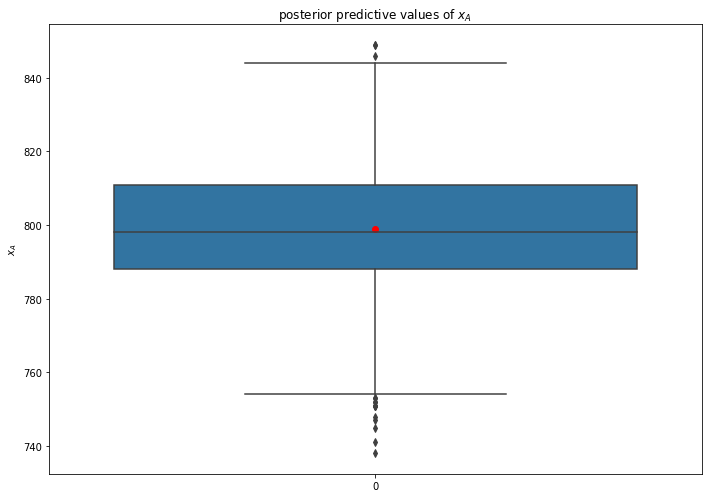
\includegraphics[width=.50\columnwidth]{early_r_ppc1_xt}\label{ppc_xt}}
	\caption[two early result box plots:]{Boxplots of posterior predictive samples of $x_A$ (1000 samples) with the actual data point of simulated $U_t$,$x_A$ value. The simulated values are shown as a red dots.}
	
\end{figure}

Figure \ref{ppc_xt} is the boxplots of posterior predictive samples of $x_A$. It is shown that the posterior predictive estimates of $x_A$ is tolerably accurate since (1) the boxplots contain actual values of $O_t$ within their lines connecting the maximum and the minimum and (2) the ranges of IQR seem modereately narrow. \\



\subsection{Early Result: Contamination of $p_A$ } 
One of the attention of this research project is to investigate how robust the model is from contaminations of the data sets. The first inspection is to check an impact of a contamination of $p_A$; what would happen if the estimation of $p_A$ is biased? It is assumed that the survey data gives us a wrong estimate of $p_A$ such that it would be underestimated or overestimated. We then want to see how the biased estimation of $p_A$ affects the estimate of $O_t$, the total overdose.\\

Both of underestimation and overestimation were conducted for the analysis. In terms of underestimation, the simulated survey data ($n_A, x_A$) was generated with $p_A=0.6$ while the true value of $p_A$ is 0.8, and all the other assumptions hold the same. That is, $x_A$ is generated from $x_A \sim Bin(n_A, 0.6)$, while $U_t$ is generated from $U_t \sim Bin(O_t, 0.8)$ for every $t$. For overestimation, the simulated survey data was generated with $p_A=0.9$ while the true value of $p_A$ is 0.8, and all the other assumptions hold the same.  \\

\subsubsection{Posterior Distribution}

\begin{figure}[htb]
	\centering
	\subfloat[ppc of $O_t$: underestimated $p_A$]{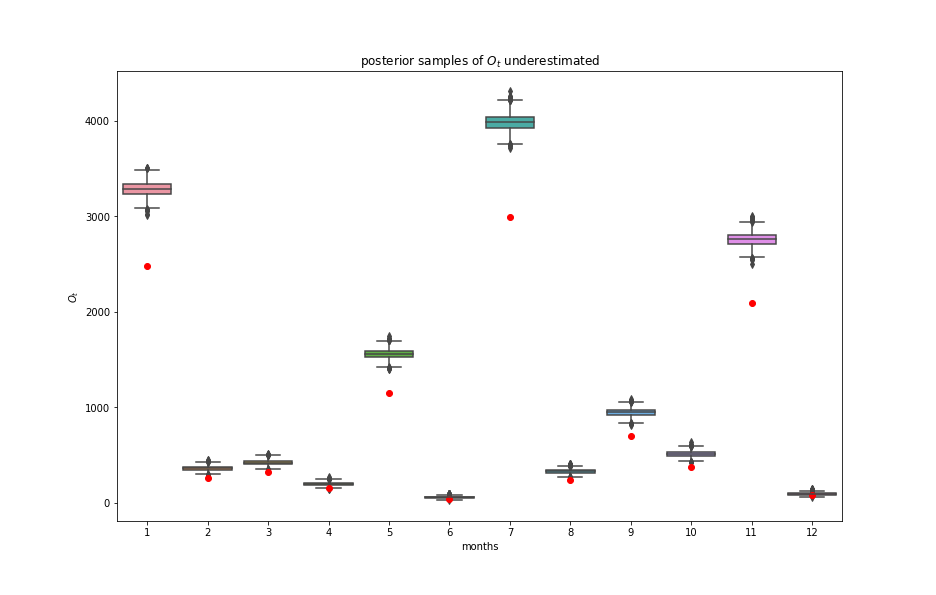
\includegraphics[width=.50\columnwidth]{early_contamination_underestimated-o_t.png}\label{under_ot}}
	\subfloat[ppc of $O_t$: overestimated $p_A$]{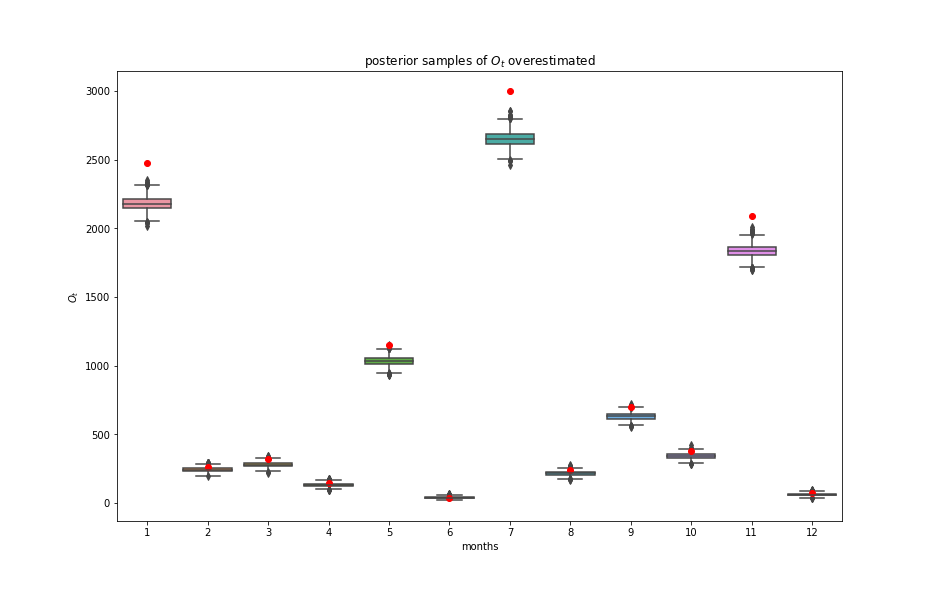
\includegraphics[width=.50\columnwidth]{early_contamination_overestimated-o_t}\label{over_ot}}
	\caption[two early result box plots:]{Boxplot of posterior samples of $O_t$ (1000 samples) where survey data is contaminated.  The actual data point of simulated $O_t$ values are shown as red dots.}
	\label{contam_ot}
\end{figure}

\normalsize 
Figure \ref{contam_ot} is the boxplots of posterior samples where $p_A$ is contaminated from the survey data. It is seen that the underestimation of $p_A$ (\ref{under_ot}) leads to an overestimation of $O_t$ as the boxplots are above the red dots. This is justifiable considering the given data sets (likelihoods) and the relationship between the two models (\ref{over_amb}); $O_t$ is generated by multiplying $U_t$ and the inverse of $p_A$ where $p_A$ is underestimated; Hence $\frac{1}{p_A}$ is overestimated which leads overestimation of $O_t$.
\begin{equation}
\label{ot.how.made}
\begin{aligned}
O_t = U_t \frac{1}{p_A}
\end{aligned}
\end{equation}
Figure \ref{over_ot} shows the opposite case. Overestimation of $p_A$ leads underestimation of the inverse of $p_A$ which causes underestimation of $O_t$. From both figures it is seen that the bias increases as the estimated values and the actual values get large.\\

\subsubsection{Posterior Predictive Check}

\begin{figure}[htb]
	\centering
	\subfloat[ppc of $U_t$: underestimated $p_A$]{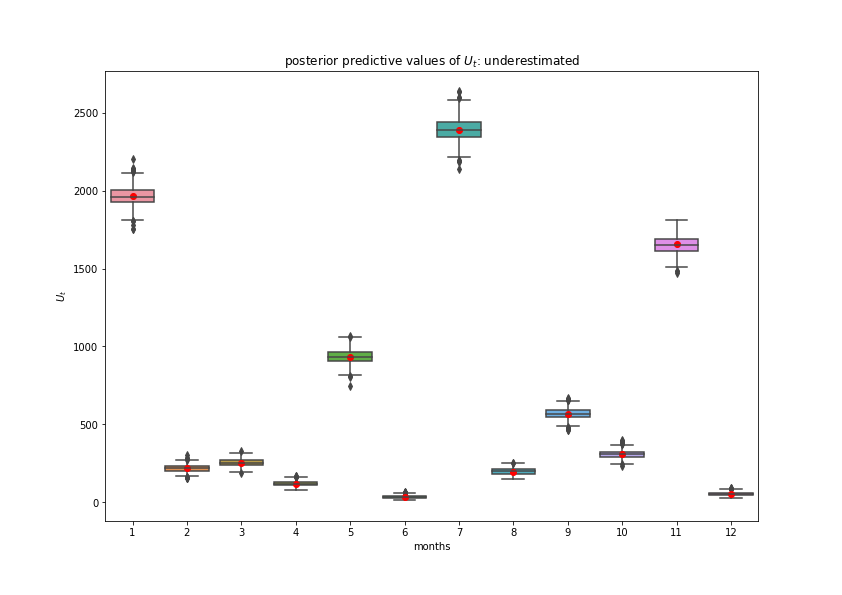
\includegraphics[width=.50\columnwidth]{early_contamination_underestimated-u_t.png}\label{under_ut}}
	\subfloat[ppc of $U_t$: overestimated $p_A$]{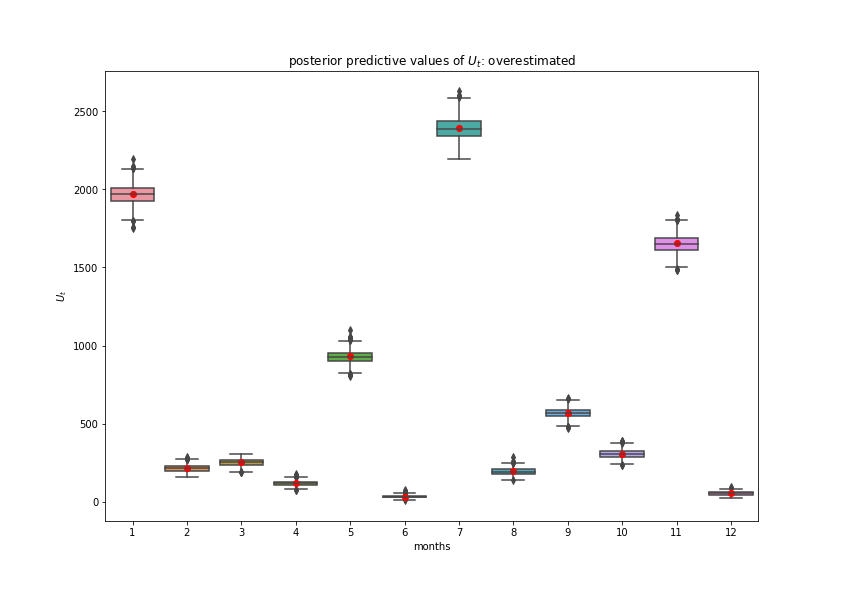
\includegraphics[width=.50\columnwidth]{early_contamination_overestimated-u_t}\label{over_ut}}
	\caption[two early result box plots:ut]{Boxplot of posterior samples of $U_t$ (1000 samples) where survey data is contaminated.  The actual data point of simulated $U_t$ values are shown as red dots.}
	\label{contam_ut}
\end{figure}


Figure \ref{contam_ut} are the boxplots of posterior predictive samples where $p_A$ is underestimated and overestimated respectively from the survey data. It is seen that the none of the contaminations of $p_A$ leads an effect  $U_t$. [Explain why is this]\\

\begin{figure}[htb]
	\centering
	\subfloat[ppc of $x_A$: underestimated $p_A$]{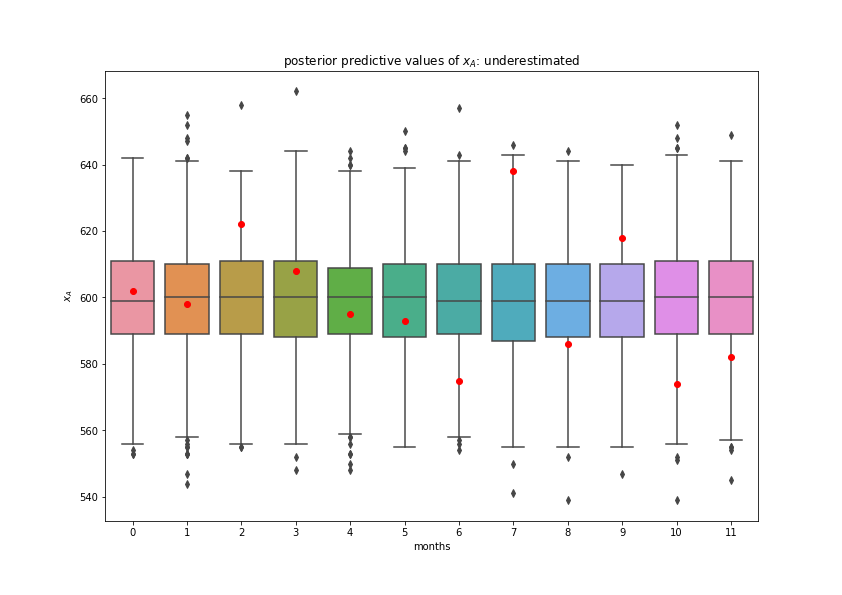
\includegraphics[width=.50\columnwidth]{early_contamination_underestimated-x_a.png}\label{under_xa}}
	\subfloat[ppc of $x_A$: overestimated $p_A$]{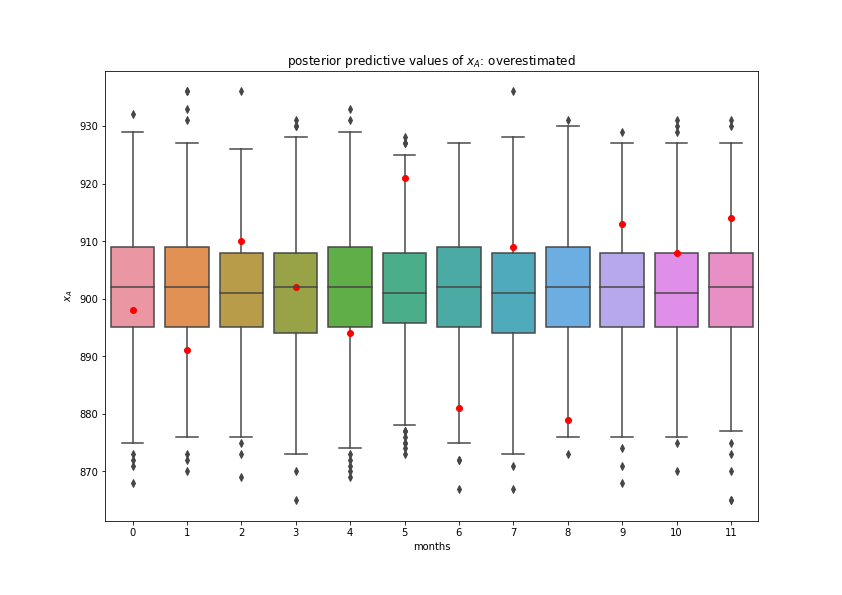
\includegraphics[width=.50\columnwidth]{early_contamination_overestimated-x_a.png}\label{over_xa}}
	\caption[two early result box plots:xa]{Boxplot of posterior samples of $x_A$ (1000 samples) where survey data is contaminated.  The actual data point of simulated $x_A$ values are shown as red dots.}
	\label{contam_xt}
\end{figure}
Figure \ref{contam_xt}  are the boxplots of posterior predictive samples of $x_A$ where $p_A$ is underestimated and overestimated respectively from the survey data. It is seen that none of the contaminations of $p_A$ leads an effect of contamination on $x_A$; the actual simulated points (red dots) are close to the medians from the two boxplots. However, notice that the range of the estimated values are different between the two boxplots; the median from Figure \ref{under_xa} is around 600 whereas the median from Figure \ref{over_xa} is around 900. [I think this should go to the previous of the previous paragraph: This is because overdose model (\ref{overdose}) does not affect the resulf from the ambulance model (\ref{ambulance}); Only the ambulance model has an effect on the overdose model.] 




\bibliographystyle{unsrt}
\bibliography{sample.bib}
\end{document}
